% !TeX spellcheck = cs_CZ
\begin{example}\label{AES:exam002} Určete vliv nenulového dynamického odporu Zenerovy diody na 
  zvlnění výstupního napětí je-li zadáno: \(U_S = \SI{14}{\volt}, u_{ripple} = \SI{100}{\mV},
  U_Z = \SI{8}{\volt}, r_Z = \SI{10}{\ohm}, R_S = \SI{50}{\ohm}, R_L = \SI{150}{\ohm}\).
  \vspace{1em}
  
  {\centering
   \begin{tabular}{cc}
     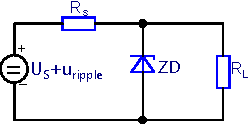
\includegraphics[width=0.4\linewidth]{stabilizator_ZD_ripple_effect.pdf}  &
     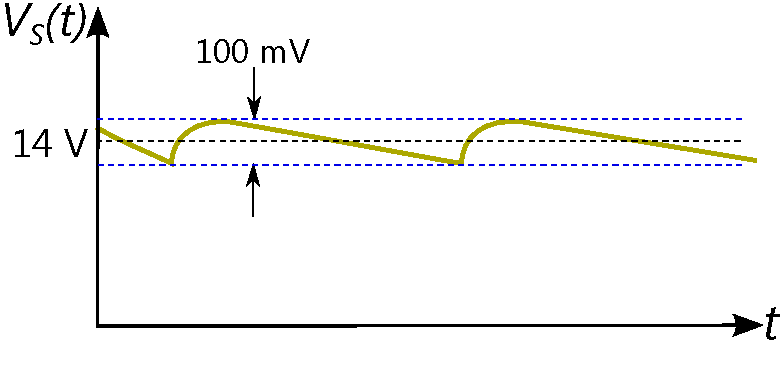
\includegraphics[width=0.5\linewidth]{stabilizator_ZD_ripple_graph.pdf}
   \end{tabular}
   \captionsetup{type=figure} 
   \captionof{figure}{K příkladu nenulového dynamického odporu Zenerovy diody na přenos zvlnění ze 
              vstupního napětí na výstupní napětí}
   \label{enz:fig_ZD_ripple}
 \par}
  \vspace{1em}
  \textbf{Řešení}:\newline Abychom stanovili velikost výstupního napětí, amplitudu zvlnění napětí 
  na zátěži a mohli také určit vliv velikosti dynamického odporu $r_z$, vyjděme z náhradního 
  lineárního obvodu na obrázku \ref{enz:fig_ZD_NLO}.
  \begin{enumerate}
    \item Stejnosměrný ekvivalentní obvod:
      \begin{align}\label{enz:eq_ZD_DC_UL}
         U_L &= U_S\frac{R_L\parallel r_z}{R_S + R_L\parallel r_z}   \nonumber \\
              + U_z\frac{R_S\parallel R_L}{r_z + R_S\parallel R_L}
             &= 2.21 + 6.32 = \SI{8.53}{\volt}
      \end{align}
    \item Střídavý ekvivalentní obvod:
      \begin{equation}\label{enz:eq_ZD_AC_UL}
        u_L = v_{ripple}\frac{r_z\parallel R_L}{R_S + r_z\parallel R_L} = \SI{16}{\mV}
      \end{equation}
      Tedy jedna šestina zvlnění vstupního napětí se přenese na výstupní svorky stabilizátoru.
  \end{enumerate}

  {\centering
   \begin{tabular}{cc}
     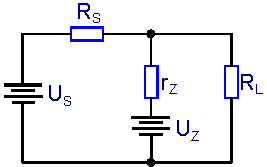
\includegraphics[width=0.4\linewidth]{stabilizator_ZD_DC_equival.pdf}
     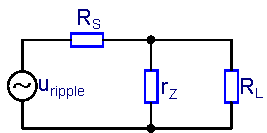
\includegraphics[width=0.4\linewidth]{stabilizator_ZD_AC_equival.pdf}
   \end{tabular}
   \captionsetup{type=figure} 
   \captionof{figure}{Stabilizátor se ZD lze pro výpočet jeho ss chování v okolí pracovního bodu  
            linearizovat pomocí NLO}
   \label{enz:fig_ZD_NLO}
  \par}
  Schopnost stabilizace je horší, čím větší má Zenerova dioda dynamický odpor $r_z$. Proto 
  musí být $r_z$ výrazně nižší, než hodnoty rezistorů $R_S$ a $R_L$ (viz rov. 
  \ref{enz:eq_ZD_AC_UL}).
\end{example}